%----------------------------------------------------------------------------------------
%       DEFINITION OF EXPERIMENTS
%----------------------------------------------------------------------------------------

\newexperiment{e0101}{Fundamental frequency estimation by eye}
\newexperiment{e0102}{Block processing}
\newexperiment{e0103}{Fundamental frequency estimator}
%\newexperiment{shorthand}{Description of the experiment}
%----------------------------------------------------------------------------------------

%	LAB BOOK CONTENTS
%----------------------------------------------------------------------------------------

% Blank template to use for new days:

%\labday{Day, Date Month Year}

%\experiment{}

%Text

%-----------------------------------------

%\experiment{}

%Text

%----------------------------------------------------------------------------------------

\labday{Exercise1 : Dienstag, 17 März 2018}

\experiment{e0101}

a)

Der Befehl audioread erhält als Argument den wav-File und liefert
einen Tupel zurück:

\begin{lstlisting}
[y1,Fs1] = audioread('speech1.wav');
[y2,Fs2] = audioread('speech2.wav');
\end{lstlisting}

Die erste Rückgabe (y1 bzw. y2) ist ein Array/Liste von Samples
(Abtastwerte).  Die zweite Rückgabe (Fs2 bzw. Fs1) liefert uns
die sampling frequency (Abtastrate, auch sampling rate siehe
Exercise 2). Mit der Abtastrate kann man sowohl den Zeitpunkt
eines Samples bestimmen ( (index des Samples in y) $\backslash$
Fs) als auch die Gesamtdauer des Signals ((length(y))
$\backslash$ Fs). Die Abtastrate beider Signale ist $16000$.    

b)

Mit dem Befehl plot kann man die Signale durch die Abtastwerte y darstellen. Für die
entsprechende Zeitstellen x muss man lediglich den Index durch die
Abtastrate nehmen:

\begin{lstlisting}
	x1 = [1:length(y1)] / Fs1;
	x2 = [1:length(y2)] / Fs2;
	figure; 
	plot(x1,y1);
	figure;
	plot(x2,y2);
\end{lstlisting}

Die Plotts sind in Abbildung \ref{img:signal1} und \ref{img:signal2} zu sehen.
Um Signale besser zu vergleichen, können wir mithilfe von subplot das Anzeigefenster zurecht splitten und Teilfenster entsprechend plotten.

\begin{figure}[H]
	\centering
	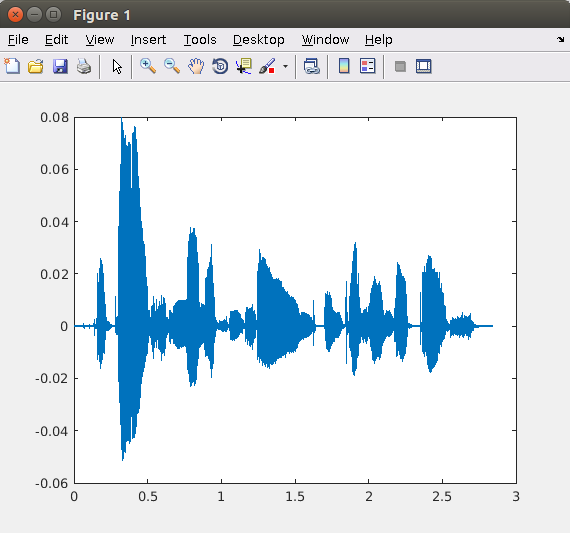
\includegraphics[width=0.6\textwidth]{./bilder/signal1.png}
	\caption{Plott des ersten Signals}
	\label{img:signal1}
\end{figure}

\begin{figure}[H]
	\centering
	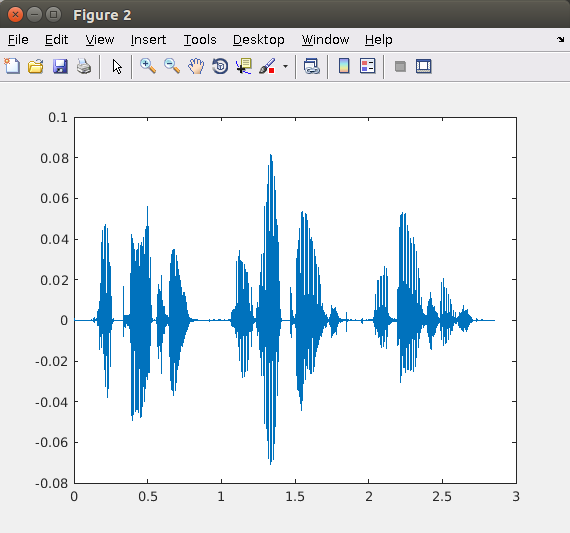
\includegraphics[width=0.6\textwidth]{./bilder/signal2.png}
	\caption{Plott des zweiten Signals}
	\label{img:signal2}
\end{figure}


Identifikation von stimmhaften etc:
\begin{itemize}
\item stimmhaft: quasi periodisch, hohe Amplituden
\item stimmlos: hat die Form von "Rauschen" 
\item silence: flach
\end{itemize}

c) 

Mithilfe von sound(lautverstärker * y(from:to),Fs) können wir den
sample-Bereich, from bis to, hören. Wenn wir der Auffassung sind, dass dieser
Bereich tatsächlich ein stimmhafter Ton ist, dann suchen wir die Grundfrequenz
wie folgt: 
\begin{itemize}
	\item Voraussetzung: Stell Zoomoption auf horizontal
	\item Zoome den entsprechenden Bereich 
	\item Zoome solange bis Wiederholungen sehbar sind
	\item Wähle eine Periode aus, messe den Abstand (Periodendauer)
	und wähle den Kehrwert als Grundfrequenz
\end{itemize}

Beispiel des zweiten deutlich erkennbaren Tons im ersten Signal:

\begin{figure}[H]
	\centering
	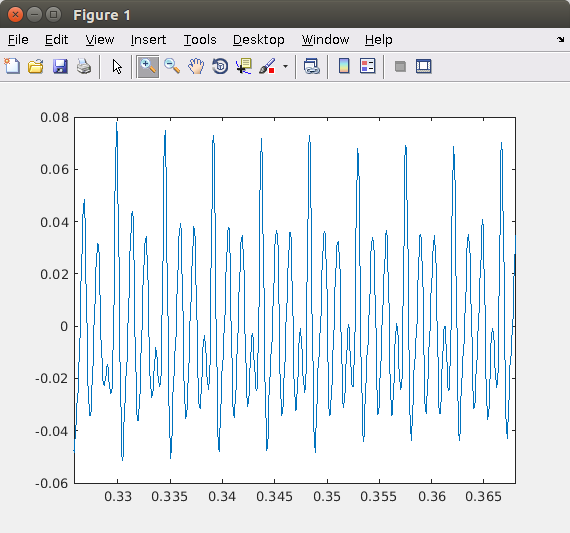
\includegraphics[width=0.6\textwidth]{./bilder/grundfrequenzsuche.png}
	\caption{Zoomen bis Wiederholung sehbar}
	\label{img:grundfrequenzsuche}
\end{figure}

\begin{figure}[H]
	\centering
	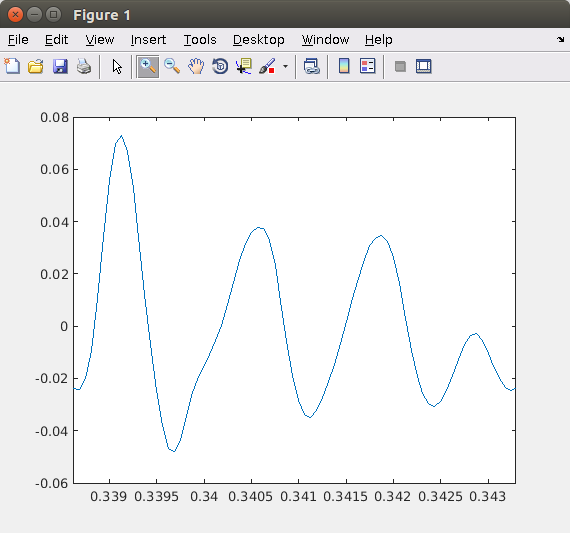
\includegraphics[width=0.6\textwidth]{./bilder/periode.png}
	\caption{Periode gezoomt}
	\label{img:periode}
\end{figure}

Die Periode beträgt aus Abbildung \ref{img:periode} geschätzt: 
$ 0.3435 s -0.3385 s = 0.005$, also einer geschätzten Grundfrequenz von $ F = 200$



% -----------------------------------------

\experiment{e0102}

Jeder Frame besteht aus einer festen Anzahl von Samples, dessen Größe durch
frame\_length in Sekunden angegeben wird.  Mit frame\_length $\cdot$ Fs erhält
man die Anzahl von Samples eines Frames. Der erste Frame fängt daher von
sekunde 0 an und endet bei Sekunde frame\_length.  Der Start des zweiten Frame wird durch
die Verschiebungen um frame\_shift nach links vom Ende des Vorgängers festgelegt.
D.h. durch die Anzahl von möglichen Verschiebung plus 1 wegen dem ersten Frame
können wir die Anzahl der benötigten Frames ermitteln:
\[
	|F| = \left \lfloor
	\frac{signal\_length - frame\_length + frame\_shift}
	{frame\_shift} \right \rfloor + 1
\]

Implementation: 
\lstinputlisting{./my_windowing.m}

% -----------------------------------------
\experiment{e0103}


% -----------------------------------------
Text


% ----------------------------------------------------------------------------------------
